% ----------------------------------------
% Chap: Literaturforschung
% ----------------------------------------
\chapter{Literaturforschung der experimentellen Techniken zur Schmierfilmdickenmessung in EHD-Kontakten}
\label{chap:literaturforschung_der_experimentellen_technik_in_ehd_schmierung}

% ----------------------------------------
% Sec: Optische Messmethoden
% ----------------------------------------
\section{Optische Messung der EHD Schmierfilmdicke}
\label{sec:optische_messung_der_ehd_schmierfilmdicke}

Viele lichtspezifische Phänomene so wie Spiegelung, Refraktion, Interferenz, etc. kann durch die Wellentheorie erklärt werden.
Einige dieser Phänomene mach Licht zu einem sehr nützlichen Werkzeug in zahlreichen Forschungsbereichen.
In diesem Kapitel werden einige Begriffe und Konzepte für die physikalische Optik kurz definiert.

% ----------------------------------------
% Sub: Lichtinterferenz
% ----------------------------------------
\subsection{Licht Interferometrie}
\label{ssec:licht_interferometrie}

Eine Lichtwelle, die eine Amplitude von $A$, eine Wellenlänge von $\lambda$ hat und die sich in $x$ Richtung mit einer Geschwindigkeit $v$ bewegt, kann durch eine Sinus- oder Cosinus Funktion beschrieben werden.
% ----------------------------------------
% Eq: Lichtwelle as sinus, cosinus function
% ----------------------------------------
\begin{equation}
        y = A \sin \cfrac{2 \pi}{\lambda} (x - v t) = A \sin (\omega t - \cfrac{2 \pi}{\lambda} x)
    \label{eq:lichtwelle}
\end{equation}
%

Das Term $x - v t$ in der Gleichung \ref{eq:lichtwelle} ist die Phase der Lichtwelle, die die Wellenposition beim Zeitpunkt $t$ angibt.
Was in der Praxis wichtig ist, ist die Phasendifferenz von zwei Lichtquellen an der gesuchten Stelle zu finden.
Wenn Licht in unterschiedlichen Medien durchdringt, wird dessen Geschwindigkeit entsprechend dem Brechungsindex der Medien verändert.
Diese Geschwindigkeitsabweichung verursacht einen Pfadunterschied $\Delta$, der in Folge zur Phasenabweichung $\delta$ führt.
% ----------------------------------------
% Eq: Licht Phasenabweichung
% ----------------------------------------
\begin{equation}
    \delta = \cfrac{2 \pi}{\lambda} \Delta
    \label{eq:lichtwelle}
\end{equation}
%

Immer wenn ein Lichtstrahl, der durch ein Medium mit einem bestimmten Brechungsindex läuft, mit einem anderen Medium mit einem anderen Brechungsindex an der Grenze ankommt, wird er teilweise reflektiert und teilweise transmittiert.
Rein nur die Reflektion allein an der Grenze resultiert auch eine Phasenverschiebung zwischen dem originalen und dem reflektierten Lichtstrahl.

Wenn zwei Lichtstrahle, die gleiche Wellenlänge sind, an einem Punkt erreichen, tritt dort das Phänomen Interferenz auf.
Durch die Überlagerung der beiden Strahlen führt es zu einer Veränderung der Amplitude bzw. Intensität des resultierenden Licht.
Wo die Intensität stärken wird, nennt man dort konstruktive Interferenz, wo die Intensität schwächen wird, nennt man destruktive Interferenz.

Diese Phänomene sind in einem Beispiel (Abbildung \ref{fig:pfadabweichung_des_lichtstrahls}), wo ein Lichtstrahl in der Luft in eine Glasscheibe mit einem Winkel $\theta$ angeht, dargestellt.
Der Brechungsindex der Luft ist $n_1$ und von der Glasscheibe ist $n_2$.
Hier wird der Lichtstrahl an der Grenze der Glasscheibe am Punkt $A$ teilweise zurück reflektiert (Pfad $ADF$) und teilweise durchgelassen (Pfad $AB$).
An der Unterseite der Glasscheibe wird er noch mal am Punkt $B$ zurück gespiegelt und am Punkt $C$ in die Luft durchdringt (Pfad $BCF'$).
Von einem Lichtstrahl gibt es jetzt zwei Lichtstrahle, die gleiche Wellenlänge sowie der originale aber wegen dem Pfaddifferenz ($ABCF' > ADF$) verschiedene Phasen haben.
% ----------------------------------------
% Fig: Licht Reflektion und Transmittion
% ----------------------------------------
\begin{figure}[htb]
    \centering
    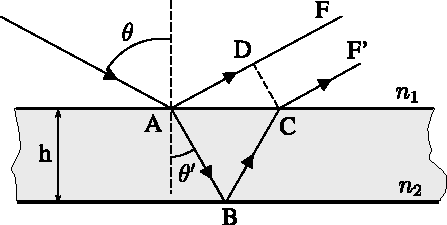
\includegraphics[]{./images/licht_interferenz_furtuna.pdf}
    \caption{Pfaddifferenz eines Lichstrahles \cite{furtuna_2011}}
    \label{fig:pfadabweichung_des_lichtstrahls}
\end{figure}
%

% ----------------------------------------
% Sub: Schmierfilmdickenmessungen mittels Lichtinterferenz
% ----------------------------------------
\subsection{Schmierfilmdickenmessungen mittels Lichtinterferenz}
\label{sub:schmierfilmdickenmessung_mittels_lichtinterferenz}

Diese Methode wurde in den frühen sechziger Jahren auf der Basis der Lichtinterferenz entwickelt und verwendet eine flache, transparente Scheibe (Glas, Saphir), die gegen eine glänzende Stahlkugel oder -rolle geladen ist (Abbildung \ref{fig:ehd_pruefsprinzip_furtuna}).
Die berührende Fläche der Scheibe ist mit einer halbdurchsichtigen Schicht (Chrom) beschichtet, so dass ein auf den Kontakt auftreffende Licht (monochrom) zweimal reflektiert wird, erstens an der Glas-Metallschicht-Grenzfläche und zweitens an der Kugel-, Rolleroberfläche.
% ----------------------------------------
% Fig: EHD Prüfsprinzip Furtuna
% ----------------------------------------
\begin{figure}[htb]
    \centering
    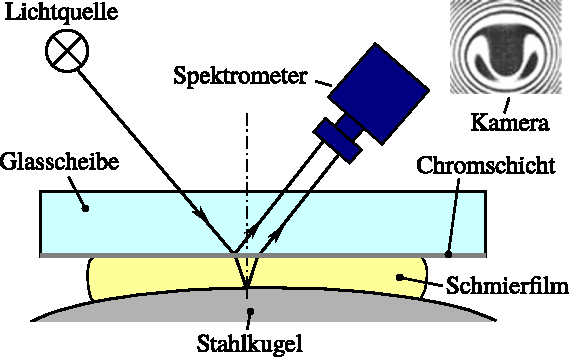
\includegraphics[]{./images/ehd_pruefsprinzip_furtuna.pdf}
    \caption{Prinzip der optischen Schmierfilmdickenmessung \cite{furtuna_2011}}
    \label{fig:ehd_pruefsprinzip_furtuna}
\end{figure}
%

Bei Rekombinaiton führt die Pfaddifferenz zwischen den reflektierten Strahlen entweder zu einer konstruktiven oder zu einer destruktiven Interferenz.
Diese Interferenzmuster hängt von der Dicke der Chromschicht und der Schmierfilmdicke ab.
Bei der bekanten Chromschichtdicke und durch entsprechende Kalibrierung lässt sich daraus die Schmierfilmdicke bestimmen.
Leider ist die Auflösung dieser Methode nicht so hoch, nur der Schmierfilm, der dicker als ein Viertel der Wellenlänge der Lichtquelle ist, ist messbar.

% ----------------------------------------
% Sub: Variante der optischen Messmethoden
% ----------------------------------------
\subsection{Variante der optischen Messmethoden}
\label{sub:variante_der_optischen_messmethoden}

\textit{Johnston et al} \cite{johnston_1991} versucht die geringe Auflösung der klassischen Methode zu überwinden.
Sein Ansatz bestand darin, eine Abstandsschicht aus Silikat mit fixierter Dicke zu verwenden, die auf der $20 nm$ Chromschicht abgelagert wurde.
Die Silikatschicht hat einen Brechungsindex, der ähnlich so wie von Mineralölen ist und wirkt als "`festes Öl"'. Sie soll die Trennung zwischen den Kontaktflächen erhöhen und dadurch ermöglicht es die Messungen von Filmen theoretisch beliebiger Dicke.
Die Vorteile der Spacer-Schicht-Methode wurden in der \textit{Ultra-Dünnfilm-Interferometrie-Methode} (UTFI) voll ausgenutzt, die weißes Licht und ein Spektrometer verwendet, um das Licht in seine Wellenlängenkomponenten zu teilen (Abbildung \ref{fig:ehd_spacer_layer_johnston}).
Die Auflösung dierser Technik liegt in der Größenordnung von Nanometern.
% ----------------------------------------
% Fig: EHD Spacer Layer Prüfsprinzip
% ----------------------------------------
\begin{figure}[htb]
    \centering
    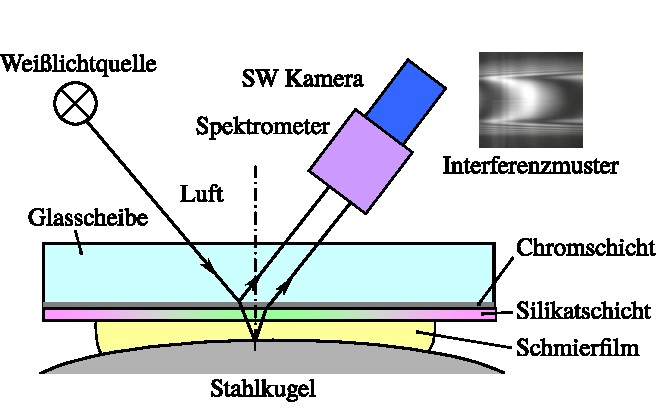
\includegraphics[]{./images/spacer_layer_methode_furtuna.pdf}
    \caption{Spacer-Layer-Methode \cite{johnston_1991}}
    \label{fig:ehd_spacer_layer_johnston}
\end{figure}
%

Eine Beschränkung der Technik der Spacer-Layer besteht darin, dass nur eine Messung von der Mitte des Kontakts aufgenommen wird.
\textit{Cann et al.} \cite{cann_1996} beschrieb die Entwicklung einer neuen Technik, die die Abbildungsfähigkeiten des klassischen optischen Verfahrens mit der UTFI-Methode kombiniert, das \textit{Spacer-Layer-Imaging-Verfahren} (SLIM) (Abbildung \ref{fig:ehd_slim_methode}).
% ----------------------------------------
% Fig: EHD SLIM Methode
% ----------------------------------------
\begin{figure}[htb]
    \centering
    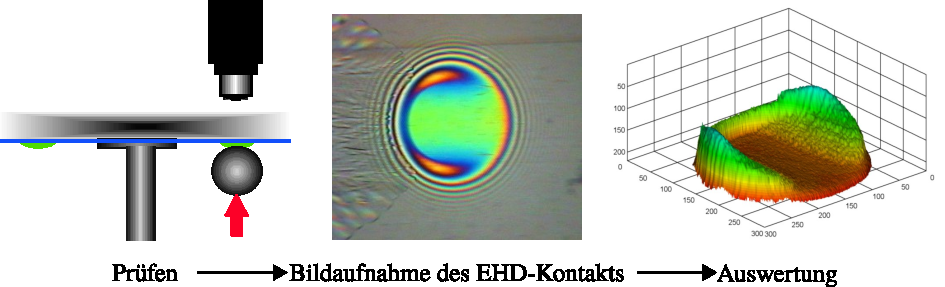
\includegraphics[]{./images/slim_methode.pdf}
    \caption{SLIM Methode \cite{ehl_broshure}}
    \label{fig:ehd_slim_methode}
\end{figure}
%

Anstatt ein Spektrometer zu verwenden, um die Wellenlänge des vom Bild eines EHD-Kontakts zurückgeworfenen Lichts zu bestimmen, benutzt SLIM eine hochauflösende RGB-CCD-Farbkamera, um ein Bild des gesamten Kontakts aufzunehmen.
Das SLIM-Softwarepaket passt die Farben im Bild anhand einer vorher festgelegten Farbraumkalibrierung an die Schmierfilmdicke an.
Das System erzeugt somit in wenigen Sekunden eine Filmdickenkarte des gesamten EHD-Kontakts.
Diese Fähigkeit macht es zu einem geeigneten Werkzeug für die Untersuchung des EHD-Kontakts in verschiedenen Bedingungen, wie zum Beispiel Fettschmierung, rauhe Oberflächen, mangelte Schmierung oder additive Grenzschichtbildung.

% ----------------------------------------
% Sec: Elektrische Methode
% ----------------------------------------
\section{Elektrische Messung der EHD Schmierfilmdicke}
\label{sec:elektrische_messung_der_ehd_schmierfilmdicke}

Neben der optischen Messmethoden gibt es noch die elektrische Messmethode zur Untersuchung der EHD-Schmierung, wie zum Beispiel Widerstand, Kapazität, Entladespannung.
Der Vorteil dieser Methode ist, dass sie direkt bei Maschinenelementen, welche aus Stahl sind, während Betrieb verwendet werden kann.
Allerdings gibt es auch Nachteile.
Die Form des Kontakts, wo die große lokale Verformung stattfindet, ist nur vermutet und stark vereinfacht.
Die hat den Einfluss auf die Widerstand-,Kapazität-Messergebnisse.
Ein Faktor noch ist die Sauberkeit des Schmierstoffes, welche schwer zu kontrollieren ist.
Generell liefern die elektrische Methode nur die mittlere Werte über den Kontaktbereich und gibt leider keine direkte Indikation der Form des Schmierfilms.

Normalerweise werden die elektrische Methoden für folgende Anwendungen verwendet:
\begin{itemize}
    \item Schmierfilmdickenmessung bei bekannten Schmierstoffen
    \item Detektion des Voll-Schmierfilaufbaus im Kontakt der rauhen Öberflächen
    \item Evaluierung des geschmierten Kontakts unter Einfluss des elektrischen Felds
\end{itemize}

% ----------------------------------------
% Sub: Widerstandmessung
% ----------------------------------------
\subsection{Widerstandmessung}
\label{sub:wiederstandmessung}

Die Widerstandmessmethode ist geeignet, um den Schmierungszustand qualitativ zu beschreiben.
Der Widerstand ist eine Indikation der direkten Berührung der Rauheitspitzen der Kontaktpartner.
Bei vollständiger Oberflächentrennung (Flüssigkeitschmierung) soll der Widerstand in theoretisch unendlich groß sein.
Zum besseren Verständnis der elektrischen Vorgängen im EHD-Kontakt wurde eine Reihe Arbeiten an unterschiedlichen Modellprüfständen und Maschinenelementen durchgeführt.

In einem System bestehend aus einer feststehenden Kugel und einem rotierenden Zylinder hat \textit{Furey} \cite{furey_1961} das Verhalten des elektrischen Widerstands untersucht.
Die Ergebnisse (Abbildung \ref{fig:resistance_vs_time_furey}) zeigten eine große Streuung des Widerstands bei Mischreibung.
Zum Beschreiben für einen isolierenden Schmierfilm definiert er einen Wert von \SI{10}{\kilo\ohm}.
In Oszilloskop erkannt er, dass es zwei Zustände des Kontaktwiderstands gabt, hoch und niedrig.
Das zeitliche Verhältnis zwischen den beiden Zuständen wird über Intervalle von \SI{10}{\milli\second} aufgenommen, ausgewertet und das Ergebnis als prozentualer Anteil des direkten Kontakt angegeben.
Mit dieser Methode konnte er berechnen, wie groß der Anteil der Festkörperkontakte in jedem Reibungszustand ist.
% ----------------------------------------
% Fig: Widerstand - Zeit Furey
% ----------------------------------------
\begin{figure}[htb]
    \centering
    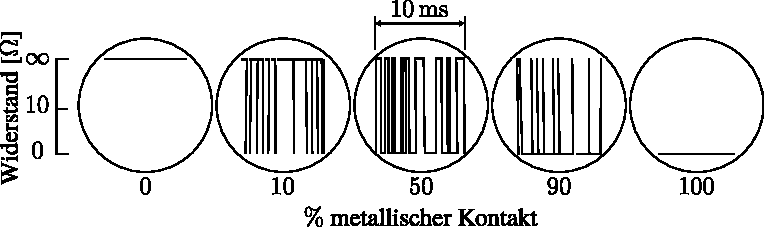
\includegraphics[]{./images/resistance_vs_time_furey.pdf}
    \caption{Der prozentuale Anteil von metallischen Kontakt \cite{furey_1961}}
    \label{fig:resistance_vs_time_furey}
\end{figure}
%

In seiner Arbeit \cite{kuhlmann_2009} verwendete \textit{Kuhlmann} zwei unterschiedliche Systeme zur Widerstandmessung.
Ein System basiert auf die \textit{Wheatstonsche} Brückenschaltung (Abbildung \ref{fig:ersatzschaltbild_messsysteme_kuhlmann} links), welche zur Vermeidung eines Tunneleffektes mit Wechselstrom gespeist wird.
Der Zusammenhang zwischen dem Widerstand $R_L$ des Lagers und der gemessenen Brückenspannung $U_m$ wird durch eine aufwändige Kalibration über variable Referenzwiderstände hergestellt.
Zur Vereinfachung der Messkettenkalibrierung und zur Verbesserung der Messempfindlichkeit bei $R_L$ mehr als \SI{1}{\kilo\ohm} setzte \textit{Kuhlmann} ein direkt messendes Trägerfrequenz-Messsystem ein (Abbildung \ref{fig:ersatzschaltbild_messsysteme_kuhlmann} rechts).
Der Widerstandszwei wird an einer hochgenauen Wechselstromquelle \SI[separate-uncertainty]{1 +- 0.2}{\milli\ampere} angeschlossen.
Aus dem Spannungsabfall über den Gesamtwiderstand ($R_V$ und $R_P$ sind bekannt) konnte er den Lagerwiderstand bestimmen.
% ----------------------------------------
% Fig: Kuhlmann Messsysteme
% ----------------------------------------
\begin{figure}[htb]
    \centering
    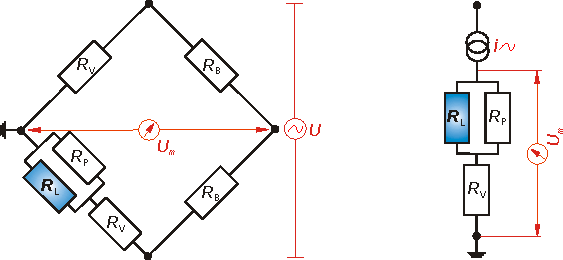
\includegraphics[]{./images/ersatzschaltbild_kuhlmann.pdf}
    \caption{Ersatzschaltbild für die Messsysteme \cite{kuhlmann_2009}}
    \label{fig:ersatzschaltbild_messsysteme_kuhlmann}
\end{figure}
%

Beide obengenannte Messsysteme wurden von \textit{Kuhlmann} bei Fettuntersuchung mit Schrägkugellagern und Kegelrollenlagern bei niedrigen Betriebstemperatur eingesetzt (Abbildung \ref{fig:schema_schraerikula_kerola_kuhlmann}).
Durch eine \SI{0.4}{\milli\meter} dicke Keramikbeschicht zwischen der Lagersitze und der Welle konnte er den Widerstand für beide Lager separat messen.
Abbildung \ref{fig:schema_schraerikula_kerola_kuhlmann} zeigt die elektrische Ersatzschaltbilder für einen Wälzkörper im Schrägkugellager und Kegelrollenlager.
Alle Wälzkörper eines Lagers sind elektrisch parallel geschaltet und der Kontakt zwischen Rollenstirn und Bord beim Kegelrollenlager muss berücksichtigt werden.
% ----------------------------------------
% Fig: Kuhlmann Test Lager
% ----------------------------------------
\begin{figure}[htb]
    \centering
    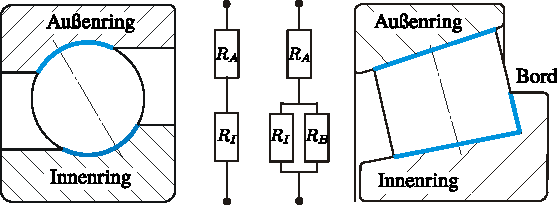
\includegraphics[]{./images/schema_schraegrikula_kerola_kuhlmann.pdf}
    \caption{Schema des Schrägkugellager- und Kegelrollenlager-Einzelkontaktes \cite{kuhlmann_2009}}
    \label{fig:schema_schraerikula_kerola_kuhlmann}
\end{figure}
%

% ----------------------------------------
% Sub: Kapazitätmessung
% ----------------------------------------
\subsection{Kapazitätmessung}
\label{sub:kapazitatmessung}

Der Vorteil bei der Kapazitätmessung ist wie bei der Widerstandsmessung die einfache Anwendung im Maschinenelement.
Es ist auch möglich bei dieser Methode quantitative Schmierfilmdickenmessung durchzuführen, welche bei resistiver Methode schwer oder unmöglich ist.

Auf Basis der Konstantstromladung hat \textit{Barz} \cite{barz_1996} ein System zur kapazitiven Schmierfilmdickenmessung im Wälzlager entwickelt.
Hier werden die Oberflächen zwischen Wälzkörpern, Außenring und Innenring bei einem trennenden Schmierfilm als Kondensator betrachtet.
Die Kapazität des einzelnen EHD-Kontaktes wird nach dem Modell von \textit{Brüser} \cite{brueser_1972} beschrieben.
% ----------------------------------------
% Fig: Brüser Modell des EHD-Kontaktes
% ----------------------------------------
\begin{figure}[htb]
    \centering
    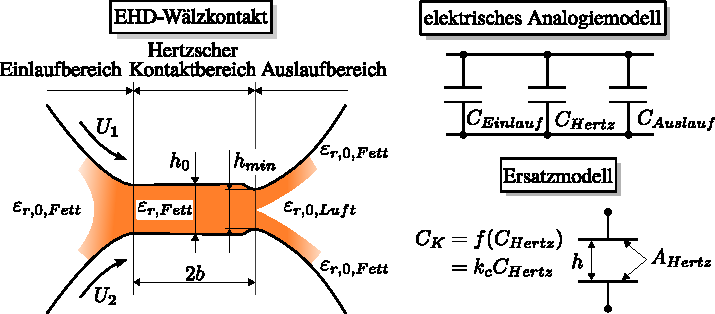
\includegraphics[]{./images/kapazitaet_schmierfilmdicke_modell.pdf}
    \caption{Kapazitives Modell eines EHD-Kontaktes \cite{barz_1996}}
    \label{fig:kapazitives_modell_eines_ehd_kontaktes}
\end{figure}
%

Im Modell von \textit{Barz} wird der EHD-Kontakt in drei Bereiche \textit{Einlaufbereich}, \textit{Hertzscher Kontaktbereich} und \textit{Auslaufbereich} geteilt und unter folgenden Annahmen betrachtet:
%
\begin{enumerate}
    \item Der Einlaufbereich ist vollständig mit Schmierstoff gefüllt
    \item Im Hertzschen Kontaktbereich herrscht es eine konstante Schmierfilmdicke $h_0$
    \item Die Einschnürung vor dem Auslaufbereich wird vernachlässigt
    \item Im Auslaufbereich haftet der Schmierstoff gleichmäßig an den Kontaktpartner an
    \item Das elektrische Feld im Hertzschen Bereich ist homogen
\end{enumerate}
%

Mit dieser Annahmen kann man die Kontaktkapazität so berechnen:
%
\begin{equation}
    C_K = C_{Einlauf} + C_{Hertz} + C_{Auslauf}
    \label{eq:kontaktkapazitaet}
\end{equation}
%
Aufgrund dem großen Einfluss und der linearen Proportional von der $C_{Hertz}$ mit der $C_K$ vereinfachte \textit{Barz} die Kontaktkapazität als:
%
\begin{align}
    C_K = f(C_{Hertz}) = k_C C_{Hertz} \\
    C_{Hertz} = \varepsilon_0 \varepsilon_r \cfrac{A_{Hertz}}{h_0}
    \label{eq:kontaktkapazitaet_vereinfach}
\end{align}
%
wobei $A_{Hertz}$ die Größe der Hertzschen Kontaktfläche, $h_0$ die zentrale Schmierfilmdicke, $\varepsilon_0$ die elektrische Feldkonstante ($\varepsilon_0 = 8,85 \cdot 10^{-15} \ \textrm{As/Vm}$) und $\varepsilon_r$ die relative Dielektrizitätskonstante ist.
In der Gleichung \ref{eq:kontaktkapazitaet_vereinfach} definierte \textit{Barz} definierte einen Umrechnungsfaktor $k_C$, welcher die $C_{Einlauf}$ und die $C_{Auslauf}$ berücksichtigt.
Er ist von den Betriebsbedingungen, dem Lager, dem Schmierstoff, der Laufzeit etc. abhängig.
Selbst ist er von der Schmierfilmdicke abhängig, da das Verhältnis zwischen $C_{Einlauf}$ und $C_{Auslauf}$ bei der Änderung der Schmierfilmdicke nicht konstant bleibt.
Für den betrachten Fall mit axial belasteten Spindellagern hat \textit{Barz} mit dem Wert $k_C = 3,5$ bestimmt.

Da die Kontakte zwischen den Wälzkörpern mit dem Außenring und dem Innenring nicht gleich sind, führte \textit{Barz} weiterhin einen Faktor $k_h$ zur individuellen Bestimmung der Schmierfilmdicke an der beiden Ringen ein.
Der ist das Verhältnis von den nach EHD-Theorie berechneten Schmierfilmdicken am Innenring $h_{EHD,i}$ und am Außenring $h_{EHD,a}$ und berechnet sich unter einer Annahme, dass die Schmierungbedingungen am Innenring und Außenring gleich sind, zu
%
\begin{equation}
    k_h = \cfrac{h_a}{h_i} = \cfrac{h_{mess,a}}{h_{mess,i}} = \cfrac{h_{EHD,a}}{h_{EHD,i}}
    \label{eq:kh_faktor}
\end{equation}
%
Schließlich berechnen sich die Schmierfilmdicken am Innenring bzw. am Außenring aus der gemessenen Gesamtkapazität $C_{ges}$ eines Lagers mit einer Wälzkörperanzahl $Z$ zu
%
\begin{align}
    h_{mess,i} &= 2 Z k_C \varepsilon_0 
                \cfrac{(\varepsilon_{r,i} A_{Hertz,i}) \left( \varepsilon_{r,a} \cfrac{A_{Hertz,a}}{k_h} \right) }
                      {(\varepsilon_{r,i} A_{Hertz,i}) + \left( \varepsilon_{r,a} \cfrac{A_{Hertz,a}}{k_h} \right) }
                \cfrac{1}{C_{ges}} \\
    %
    h_{mess,a} &= k_h h_{mess,i}
\end{align}
%


% ----------------------------------------
% Sec: Alternative Methoden
% ----------------------------------------
\section{Alternative EHD Schmierfilmdicke Messmethoden}
\label{sec:alternative_messmethoden}

% ----------------------------------------
% Sub: Taktile Messung
% ----------------------------------------
\subsection{Taktile}
\label{sub:taktil}

Um den Schmierfilmaufbau in Axialzylinderrollenlagern unter der Annahme, dass die zentrale Schmierfilmdicke $h_0$ eine gleiche Verschiebung zwischen Wälzkörpern und Lagerringen verursacht, zu untersuchen, hat \textit{Walbeck} in seiner Arbeit \cite{Walbeck_2004} einen modifizierten FE8-Prüfkopf (FE8-SDM) benutzt (Abbildung \ref{fig:fe8_sdm_walbeck}).
% ----------------------------------------
% Fig: Walbeck FE8 Prüfkopf
% ----------------------------------------
\begin{figure}[htb]
    \centering
    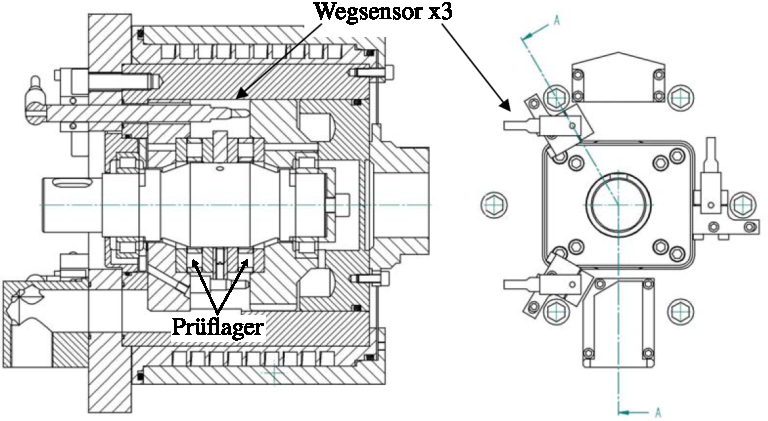
\includegraphics[]{./images/fe8_sdm_walbeck.pdf}
    \caption{FE8-SDM Prüfkopf \cite{Walbeck_2004}}
    \label{fig:fe8_sdm_walbeck}
\end{figure}
%

In der neben einander Anordnung sollen die Schmierfilme in zwei Prüflagern eine Gesamtverschiebung von $x_{ges} = 4  h_0$ verursachen.
Zur Messkette, die mit einem maximalen Messfehler von \SI{0,9}{\micro\meter} aufweist, gehören die drei hochauflösende induktiv Wegaufnehmer.
Wird es auf den einzelnen Schmierspalt bezogen, reduziert sich der maximal mögliche Fehler auf \SI{0,23}{\micro\meter}.
Da die Erwärmung im Schmierspalt kann zum Messfehler verursachen, führte \textit{Walbeck} die Messungen bei relativ geringen Kontaktpressungen (\SIrange{419}{593}{\mega\pascal}) durch.
Allerdings ist die Wärmeentwicklung durch Lagerreibung nicht vermeidbar und dadurch ist eine absolute Schmierfilmdickenmessung wegen Wärmedehnung in Bauteilen nicht möglich.
Abhilfe zählt hier die Differenzmessung der Verschiebung zwischen Stillstand und Betriebsdrehzahl.
Um die thermische Effekte auf die Messergebnisse gering zu halten, soll die Drehzahländerung innerhalb einer halbe Sekunde dauern.
Zusätzlich wurde die Wegmessungen von Winkelstellung der Welle getriggert, um der Fehler wegen Formtoleranzen der Lagerscheiben zu vermeiden.

Ein ähnliches System wurde von \textit{Kuhlmann} \cite{kuhlmann_2009} zur Schmierfilmdickenmessung in Schrägkugel- und Kegelrollenlagern eingesetzt.
Wegen der Geometriedifferenz zwischen zwei Lagerbauarten und dem Axialzylinderrollenlager ist die axial Verschiebung in diesem Fall eine Funktion von dem Druckwinkel $\alpha$.
Für das Kegelrollenlager muss Zusätzlich den Kontakt zwischen Rollenstirnfläche und Innenringbord berücksichtigt werden.
% ----------------------------------------
% Fig: Kuhlmann FE8
% ----------------------------------------
\begin{figure}[htb]
    \centering
    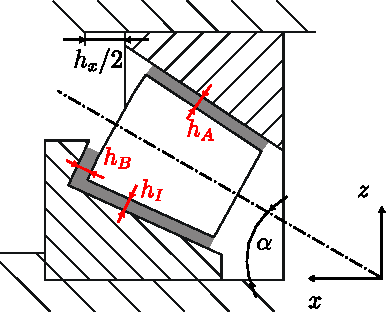
\includegraphics[]{./images/kerola_kuhlmann.pdf}
    \caption{Schmierfilme im Kegelrollenlager \cite{kuhlmann_2009}}
    \label{fig:kerola_kuhlmann}
\end{figure}
%

Die Schmierfilmdickenmessungen wurden von \textit{Kuhlmann} während des Abbremsvorgangs von der Betriebsdrehzahl auf eine minimale Drehzahl von $n_0 =$ \SI{0.5}{\per\minute} innerhalb \SI{1.5}{\second} durchgeführt (Abbildung \ref{fig:differenzmessung_kuhlmann}).
% ----------------------------------------
% Fig: Kuhlmann Messung während des Abbremsvorgangs
% ----------------------------------------
\begin{figure}[htb]
    \centering
    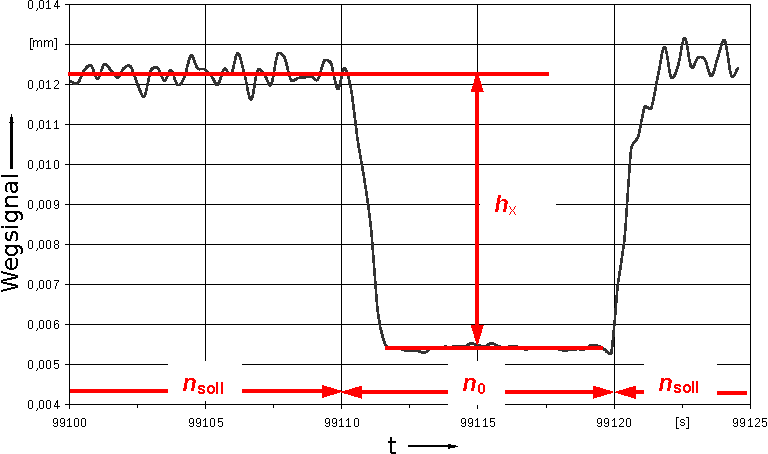
\includegraphics[]{./images/differenzmessung_kuhlmann.pdf}
    \caption{Messung während eines Abbremsvorgangs \cite{kuhlmann_2009}}
    \label{fig:differenzmessung_kuhlmann}
\end{figure}
%

Anstatt von der Winkelstellung der Welle getriggert wurde vor jedem Versuch eine Kalibrierkurve der Wegsensoren, in die die gemittelten Planlaufabweichungen zwischen den Lagern und der Prüfwelle in Abhängigkeit mit der Wellenstellung dargestellt werden, bei der Drehzahl $n_0$ aufgenommen (Abbildung \ref{fig:kalibrierkurve_kuhlmann}).
Bei der Auswertung der Schmierfilmdicke bei einer Betriebsdrehzahl findet eine Korrektur der gemessenen Verschiebung an der jeweiligen Wellenposition anhand der Kalibrierkurve statt.
% ----------------------------------------
% Fig: Kuhlmann Kalibrierkurve
% ----------------------------------------
\begin{figure}[htb]
    \centering
    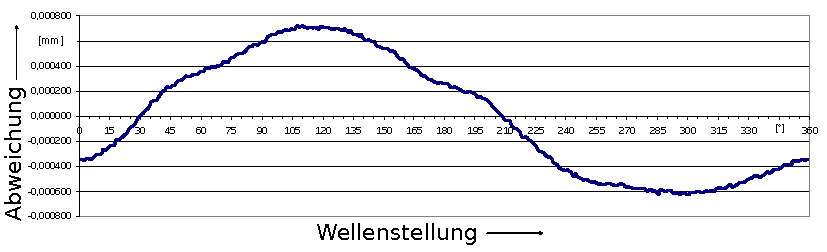
\includegraphics[]{./images/kalibrierkurve_kuhlmann.pdf}
    \caption{Kalibrierkurve \cite{kuhlmann_2009}}
    \label{fig:kalibrierkurve_kuhlmann}
\end{figure}
%

% ----------------------------------------
% Sub: Ultrashall Messung
% ----------------------------------------
\subsection{Ultraschall}
\label{sub:ultraschall}

\textit{Dwyer-Joyce et al.} \cite{dwyer-joyce_2011} beschrieben ein neues Verfahren zur Dickenmessung einer zwischen einer Stahlkugel und einer Stahlscheibe liegende Flüssigkeitsschicht mittels der Reflektion des Ultrashalls.
Diese Reflektion hängt von der Ultraschallfrequenz, den akustischen Eigenschaften der Flüssigkeit bzw. der Festkörper und der Schichtdicke ab.
Wenn die Wellenlänge des gesendeten Impulses viel größer als die Dicke der Flüssigkeitsschicht ist, wird die Antwort durch die Steifigkeit der Schicht bestimmt.
Wenn die Wellenlänge ähnlich sowie die Schichtdicke ist, wird die Wechselwirkung vom Ultraschall mit der Flüssigkeit durch sein Resonanzverhalten gesteuert.
Durch das Vergleich des Frequenzspektrums des reflektierten Impulses mit dem des gesendeten Impulses ermöglicht die Bestimmung der Schmierfilmdicke.
Die Messmethode von \textit{Dwyer-Joyce} war in der Lage, Filme im Bereich von \SIrange{50}{500}{\milli\meter} zu messen.
Der schematischer Aufbau des Ultraschall-Prüfstands zur Schmierfilmdickenmessung ist in Abbildung \ref{fig:ultrashall_pruefstand_dwyer-joyce} zu nehmen.
% ----------------------------------------
% Fig: Dwyer-Joyce Ultrashall test rig
% ----------------------------------------
\begin{figure}[htb]
    \centering
    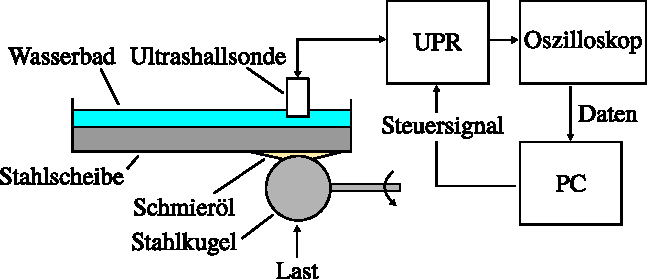
\includegraphics[]{./images/ultrashall_pruefstand_dwyer-joyce.pdf}
    \caption{Schematischer Aufbau der Ultraschall-Prüfstand \cite{dwyer-joyce_2011}}
    \label{fig:ultrashall_pruefstand_dwyer-joyce}
\end{figure}
%

Ein Schmierfilm-Überwachungssystem an einem Rillenkugellager mittels Ultraschall wurde von \textit{Zhang et at.} in seine Arbeit \cite{zhang_2006} beschrieben (Abbildung \ref{fig:ultrashall_rikula_zhang}).
Eine Hochfrequenz-Ultraschallsonde ist am statischen Außenring des Lagers montiert.
Die Sonde ist auf die Kugel-Laufbahn fokussiert und wird verwendet, um die Reflektion-Koeffizienten des Schmierstoffes in der Kontaktellipse wischen Lagerkomponenten zu messen.
Der Reflektion-Koeffizient kennzeichnet den Schmierfilm und kann daraus seine Dicke berechnet werden.
Ein optisches Triggersystem ermöglicht mehrere Messungen, wenn jeder geschmierte Kontakt sich an der Messstelle vorbeibewegt.
Drei Verunreinigungsmaterialien (Aceton, Wasser und Sand) wurden separat zu dem Schmiermittel gegeben, um das Versagen des Lagers zu initiieren.
Diese Zugabe simuliert allgemeine Fehlermechanismen, die unter realen Bedingungen auftreten können.
    Alle Ergebnisse, wie zum Beispiel die Schwingung, die Temperatur, die Ultraschall-Reflektion-Koeffizienten wurden unter diesen drei Fehlerszenarien aufgenommen und die lieferten wertvolle diagnostische Informationen über die Fehler sowie Frühschadenmeldung.
% ----------------------------------------
% Fig: Zhang Ultraschall Versuch am Rikul 6016
% ----------------------------------------
\begin{figure}[htb]
    \centering
    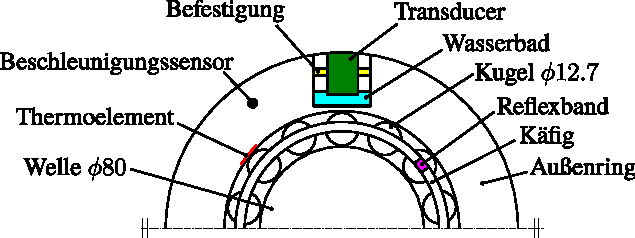
\includegraphics[]{./images/ultrashall_rikula_zhang.pdf}
    \caption{Schmierfilm-Überwachungssystem mittels Ultraschall \cite{zhang_2006}}
    \label{fig:ultrashall_rikula_zhang}
\end{figure}
%

% ----------------------------------------
% Sub: Laserinduzierte Messung
% ----------------------------------------
\subsection{Laserinduzierte Fluoreszenz}
\label{sub:laserinduzierte_fluoreszenz}

\textit{Jones et al.} beschrieb in seiner Arbeit \cite{jones_2001} die Kalibrierung einer Technik, die auf Basis der Laserinduzierten Fluoreszenz zur quantitativen Messungen von industriellen Beschichtungen mit einer Dicke von \SIrange{10}{20}{\nano\meter} ermöglicht.
Wachsfilme, die mit einem fluoreszierenden Rhodaminfarbstoff dotiert waren, wurden durch ein Elektrospray-Verfahren auf eine Seite der aluminiumbeschichteten Glasscheibe aufgebracht.
Mit einem optischen Profilometer mittels Lasertriangulation wurden die Filmdicken von \SIrange{220}{450}{\milli\meter} ermittelt.
Die emittierte Fluoreszenz wurde unter der Verwendung einer fasergekoppelten Sonde mit Laseranregung und Spektraldetektion aufgenommen.
Die Fluoreszenzemission wurde wegen der Aluminiumschicht um zehnfach reduziert.
Die Kalibrierung lieferte gute Ergebnisse, die in Übereinstimmung mit den aus Volumenmessung im Beschichtungsprozess geschätzten Filmdicken sind.
% ----------------------------------------
% Fig: Schematische Aufbau der Kalibrierung mit Profilometer
% ----------------------------------------
\begin{figure}[htb]
    \centering
    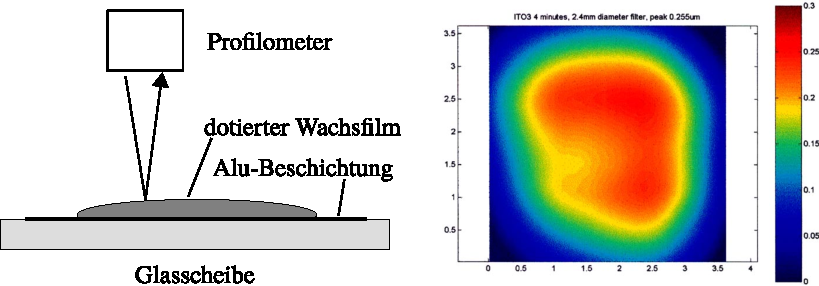
\includegraphics[]{./images/schematic_profilometer_and_scan_result_jones.pdf}
    \caption{Schematische Aufbau der Kalibrierung mit Profilometer (links) und deren Scan-Ergebnis (Dickenkarte) (rechts) \cite{jones_2001}}
    \label{fig:aufbau_laserinduzierte_kalibrierung_jones}
\end{figure}
%
